% As a general rule, do not put math, special symbols or citations
% in the abstract
\begin{abstract}
%	Many of today's safety-critical systems are reactive, embedded systems. Their internal behavior is usually represented by state-based models. Furthermore, as the tasks carried out by such systems are getting more and more complex, there is a strong need for compositional modeling languages. Such modeling formalisms start from the component-level and use composition to build the system-level model as a collection of simple modules.
%	There are a number of solutions supporting the model-based development of safety-critical embedded systems. One of the popular open-source tools is Yakindu, a statechart editor with a rich language and code generation capabilities. However, Yakindu so far lacks support for compositional modeling.
%	This paper proposes a formal compositional language tailored to the semantics of Yakindu statecharts. We propose precise semantics for the composition to facilitate formal analysis and precise code generation. Based on the formal basis laid out here, we plan to build a complete tool-chain for the design and verification of component-based reactive systems.
\end{abstract}

% For peer review papers, you can put extra information on the cover
% page as needed:
% \ifCLASSOPTIONpeerreview
% \begin{center} \bfseries EDICS Category: 3-BBND \end{center}
% \fi
%
% For peerreview papers, this IEEEtran command inserts a page break and
% creates the second title. It will be ignored for other modes.
\IEEEpeerreviewmaketitle

\section{Introduction}
\label{sec:introduction}
Statecharts \cite{Harel:1987:SVF:34884.34886} are a popular formalism to describe the behavior of reactive systems, which process stimuli from the environment and react with respect to their internal states. Statecharts introduce complex elements to aid the modeling of such systems, e.g., variables, hierarchical state refinement, history states and complex transitions (e.g., inner transitions).

The requirements such systems have to meet are getting more complex, which can result in very large system models, encumbering verifiability, maintenance and extensibility. A well-known solution for managing complexity is decomposition. In case of statecharts, one way of decomposition is to define individual reactive components that, by means of some communication, realize a more complex behavior. There are a number of modeling tools that aim to support this practice with various model-driven software development techniques such as code generation and verification.

The Gamma Statechart Composition Framework is one such tool, providing a layer for composing individual statechart components (possibly coming from other tools) while extending the capabilities of automatic code generation and verification and validation (V\&V). In this paper, we introduce the new composition language of Gamma that enables the hierarchical mixing of different composition semantics, with a focus on features and modeling aspects.

\textbf{Asynchronous-reactive:} Such models represent a set of components that are executed independently. Asynchronous components communicate with each other by means of messages and message queues. This semantics is convenient when decomposition is both logical and physical, \eg for the design of communicating microservices running in different processes.
	
\textbf{Synchronous-reactive:} A synchronous model represents a coherent unit with a single functionality consisting of concurrently (but not independently) running components. Contained components communicate in a synchronous manner using signals. This semantics is suitable for the logical decomposition of systems or the modeling of hardware-related designs.
	
\textbf{Cascade:} Cascade models represent a set of filters that are applied sequentially to derive an output from an input. Like synchronous-reactive components, cascade components also facilitate the logical decomposition of a problem, but it focuses more heavily on process-like models. Therefore, this model supports the design of adapters, runtime monitors and units with a batch-like execution.

The rest of the paper is structured as follows. Section~\ref{sec:related-tools} presents a short summary of tools that inspired the design of the composition language. The elements of a the language itself and an example are introduced in Section \ref{sec:composition-language}. Finally, Section \ref{sec:conclusion} provides concluding remarks and ideas for future work.

\section{Related Tools}
\label{sec:related-tools}

\ptolemy\footnote{\url{http://ptolemy.eecs.berkeley.edu/}} \cite{ptolemy,ptolemy2} is an open-source software framework, aiming to support
the modeling of hierarchical composite systems. It supports system design with numerous component variants and communication semantics. Communication semantics of interactive components are determined by \emph{directors}, which are responsible for defining a \emph{model of computation} on a particular hierarchy level. Various directors (e.g., process network, synchronous data flow
or synchronous reactive) through different hierarchy levels can be combined, facilitating the design of complex model behavior. One of the main strengths of Ptolemy II is the simulation capability of designed models. However, source code generation from models is not supported and it does not provide formal verification capabilities either.

BIP\footnote{\url{http://www-verimag.imag.fr/Rigorous-Design-of-Component-Based.html?lang=en}} \cite{bip,bip3} is a modeling framework that focuses on the formal definition of heterogeneous systems.
BIP offers a language to define hierarchical composite models, where the interactions of constituent components are based on \emph{synchronization}. BIP defines a clear operational semantics that describes the behavior for both atomic components (transition system model) and compound components (rigorous interaction rules of contained components). BIP offers a comprehensive tool set, which provides model transformers for third-party models, e.g., MATLAB/Simulink, code generators to produce C/C++ code, and formal
verification capabilities of defined BIP models.

Stateflow\footnote{\url{https://www.mathworks.com/products/stateflow.html}} \cite{stateflow} is a commercial framework that supports the modeling of
reactive systems. Stateflow supports the design of composite
statecharts by combining
statechart diagrams with flowchart diagrams and providing various scheduling
algorithms. Furthermore, Stateflow supports the simulation, validation and verification of created models as well as source code generation. Stateflow is a mature software with professional
support. Unfortunately, as Stateflow is a commercial product, its study and extension is cumbersome, which is not favorable in research context. Also, commercial licenses are expensive.


%\section{The Gamma Statechart Language}
%\label{sec:statechart-language}
%The goal of the \gamma\ statechart language is to support the rigorous design of reactive
%systems while providing conventional facilities of modern statechart languages. To support
%strictness, a well-defined semantics is needed. The language is given a denotational semantics
%described in \cite{graics-bence-bsc} by mapping gamma model constructions to the elements of a formal timed
%automaton implementation. The most important elements of the language are presented in this section using a simple \emph{timer} statechart capable of measuring time.
%
%The execution of the statechart starts in the \textsl{Idle} state, with the \textsl{elapsedTime} variable set to $-1$. When a \textsl{start} event is received on its \textsl{control} port, it changes its state to \textsl{Measuring}, where the incoming \textsl{tick} events are counted using a loop transition. When a \textsl{stop} event is received, the statechart goes back to state \textsl{Idle} while storing the elapsed number of ticks in variable \textsl{elapsedTime}. The measuring process can be restarted with an additional \textsl{start} event.
%\begin{lstlisting}
%statechart Timer [
%  // Port for communication
%  port control : provides Control
%] {
%  var elapsedTime : integer := -1
%  // Transition without trigger
%  transition from Initial to Idle 
%  // Transitions with triggers
%  transition from Idle to Measuring
%    when control.start / assign elapsedTime := -1
%  transition from Measuring to Measuring
%    when control.tick && !(control.stop)
%  transition from Measuring to Idle
%    when control.stop
%  // Main region
%  region main {
%    // Initial state
%    initial Initial
%    // Simple state
%    state Idle
%    // Simple state with entry action
%    state Measuring {
%      entry / assign elapsedTime := elapsedTime + 1
%    }		
%  }
%}
%\end{lstlisting}
%
%Statecharts communicate with their environment via \textsl{ports} using \textsl{events}. A port realizes an \textsl{interface} in either required or provided mode, which determines the event types that can be dispatched or received through the particular port. The language supports the definition of \textsl{variables} with the following types: integer, natural, real, boolean and enumeration types. Variables can be used in guard expressions and assignment expressions of \textsl{transitions}. Events of ports can also be raised by transitions.
%
%One of the unique features of the \gamma\ statechart language is the \textsl{complex trigger}. A complex trigger, consisting of simple triggers, can describe the relation
%of multiple triggers as logical relations. A complex trigger may initiate a particular execution only if the corresponding logical relation is evaluated to true. Furthermore, an execution can be
%initiated on the absence of a certain event.
%
%\textsl{Region} is the container element of node elements. A region can either be a top region, contained by a statechart or a subregion,
%contained by a composite state. A region must contain a single entry state, which can be an \textsl{initial state} (no history), a \textsl{shallow history} or \textsl{deep history state}. \textsl{States} can have \textsl{entry} and
%\textsl{exit events}, which specify different actions that have to be taken when the state is activated
%or deactivated, respectively. \textsl{Composite states} extend simple states with the ability of containing
%one ore more regions. If a particular state contains multiple regions, they are parallel.

\section{The Gamma Composition Language}
\label{sec:composition-language}
The \gamma\ composition language supports the definition of communicating composite models
built from individual reactive components. The design of composite systems starts with the definition of interfaces, which define the possible event types that can be transmitted between components. The interfaces then can be realized by ports of components, which can be connected, thus enabling communication. Communicating components can be wrapped by composite models, creating an independent composite reactive unit with rigorously defined interaction patterns.

\subsection{Communication Elements}
\label{sec:communication-elements}
Interfaces serve as contracts between
interacting components of \gamma\ models. These contracts apply to the ability of dispatching
and receiving certain events. Events represent occurrences of some importance. Directions of events can be in, out or in-out;
the latter represents events that can be used as both in and out events. Events can contain
parameter declarations, which provide additional information about the corresponding event. An example interface definition can be seen below.
\begin{lstlisting}
interface LightCommands {
  out event displayRed
  out event displayGreen
  out event displayYellow
  out event displayNone
}
interface PoliceInterrupt {
  out event police
}
\end{lstlisting}

Ports serve as endpoints of component instances in a composite component model,
through which events can be dispatched or received. In \gamma\ models, communication between component
instances always happens through ports. Events are either called signals in case of
synchronous components or messages in case of asynchronous components. Each port realizes
a single interface in either provided or required mode. In provided mode ports dispatch and receive events according to the direction specified in the event declarations. In case of required mode, interfaces are ``turned inside out'', i.e., events declared with the direction in will be
dispatched, and events declared with the direction out will be received through such ports. Note that if two ports realize the same interface, one of them in provided mode, the other
one in required mode, they can be connected since the direction of the events would match. Note that
the realization mode does not specify a single direction in which events are transmitted
through the particular port – dispatch and reception can be mixed in both cases. A port is considered as a broadcast port if the interface realization mode is provided and
the realized interface contains only out events. Unlike other ports, a broadcast port can
be connected to multiple ports realizing the same interface in required mode.

The concept of ports realizing interfaces in providing or requiring modes may be unusual to
some designers, since ports usually support one-way event transmission in modern modeling
languages. Our goal with this solution is to investigate the possibilities residing in interface-based
communication in the domain of reactive systems. On the other hand, it is possible to
use only out events on every interface -- then provided mode is ``output'' mode and required
mode is ``input'' mode.

\subsection{Components}
Components serve as types of component instances in \gamma\ composite models. As introduced in \ref{sec:communication-elements}, each component defines one or more ports through which communication can take place, as presented in the following snippet.
\begin{lstlisting}
sync Crossroad [
  port police : requires PoliceInterrupt,
  port priorityLightOutput : provides LightCommands,
  port secondaryLightOutput : provides LightCommands
]
\end{lstlisting}

A component can be either atomic, which wraps a single statechart, or composite, which wraps one or more component instances. Statecharts can be defined using the \gamma\ Statechart Language, presented in \cite{graics-bence-bsc}. Each composite component type -- asynchronous-reactive, synchronous-reactive and cascade -- adopts a rigorous computational semantics. However, they are always based on the same basic modeling elements -- component instances, port bindings and channels -- which can be extended by element set of the particular component type.

Component instances are individual reactive elements with internal state, capable of receiving
and dispatching events through ports. Each component instance refers to a single
component, serving as its type, which determines the ports on which
the component instance shall be able to communicate as well as the internal states it shall
be able to assume and the transitions it shall be able to fire. Component instances can
be either atomic or composite. The instance is atomic if the corresponding component is a
statechart definition and composite if it refers to a composite component. This enables the
hierarchical composition of \gamma\ models.

\begin{lstlisting}
// Component instances with component types
component controller : Controller
component priorityLight : TrafficLight
component secondaryLight : TrafficLight
\end{lstlisting}

Port binding The port binding element is responsible for the connection of the exterior
ports of a composite component and the ports of constituent component instances. Therefore,
it refers to a single port of a component instance. Owing to this design, all events received on the particular composite component port will be transmitted to the port of the associated
component instance, and all the events dispatched through the particular instance port will
be transmitted to the composite component port.

\begin{lstlisting}
// Binding component ports to internal ports
bind police -> controller.policeInterrupt
bind priorityLightOutput -> priorityLight.lightCommands
bind secondaryLightOutput -> secondaryLight.lightCommands
\end{lstlisting}

Channels are responsible for the connection of component instance ports, enabling event flow between ports. There are two types of channels, simple channel and broadcast channel. Simple channels support the connection of a single port providing and a single port
requiring the same interface. As explained in Section \ref{sec:communication-elements}, this design is valid and safe
since they handle the same events with appropriate directions. Broadcast channels support sending events to multiple target ports. Such channels refer
to \textit{1)} a single broadcast port and \text{2)} multiple ports requiring the same interface as the
one the broadcast port provides. In this case the direction of event transmission is
determined: the broadcast port dispatches events and all the other ports connected to
it receive them.

\begin{lstlisting}
// Channel definitions connecting internal ports
channel [controller.priorityControl] -o)-
  [priorityLight.control]
channel [controller.secondaryControl] -o)-
  [secondaryLight.control]
\end{lstlisting}

\subsection{Composite Component Variations}
Composite components can be classified into \emph{synchronous} and \emph{asynchronous components} regarding their execution semantics.

\subsubsection{Synchronous Components}
Synchronous components represent models that communicate
in a synchronous manner using \emph{signals}. Synchronous components do not run independently, but their
execution is scheduled by a scheduler, e.g., a wrapping asynchronous component. When executed, synchronous components process incoming signals
and produce output signals in accordance with their internal states. Output signals are
produced for a single execution period only, i.e., another execution might produce different
output signals overwriting the output signals of the previous one. Synchronous components in \gamma\ are the followings:  statechart definitions, synchronous composite
components and cascade composite components.

\paragraph{Synchronous composite component} The execution of a synchronous composite component
conforms to a turn-based semantic. A turn is called a \emph{cycle}. In each cycle all component instances of the particular composite component are executed. Although the order of the execution of the component instances is not defined, it is fixed, therefore they are executed in the same order in each cycle. This does not cause a loss of generality, as components cannot affect each other in a single execution cycle: if a component instance produces a signal that another component instance receives, the receiver will get it in the next cycle. If a single component instance is executed it may \textit{1)} process all signals received in the last execution turn, \textit{2)} assume a new state according to the processed signals (new state configuration, new variable values) and \textit{3)} produce signals that can be received by components (others or itself).

\paragraph{Cascade composite component} Cascade composite components contain the same elements
as synchronous composite components, but their execution semantics is different. The
execution of a cascade composite component also consist of cycles. In a single cycle all components
of the particular composite component are executed according to a topological ordering
based on channels. If a component is executed, it processes all incoming signals and produces
signals in accordance with its internal state. However, the signals are processed in the same
execution cycle by receivers, and not in the next one as it is specified in synchronous composite
components. Therefore, in cascade composite components the flow of signals is one-way:
component instances earlier in the ordering transmit signals to the ones that are later, in
accordance with channel definitions. This structure ensures that a component can process all
signals it receives in a single cycle.

As a summary of synchronous composite models, the following code snippet defines an example Crossroad model, which is responsible for the control of two traffic lights at a crossroad. It has three ports for communication and contains three statechart component instances: two traffic lights and a controller unit. The ports of the composite component are bound to the ports of the component instances. Furthermore, channel definitions enable the communication (flow of signals) between the controller unit and the controlled traffic light components. Figure \ref{fig:crossroads-composite-model} presents the defined Crossroad model graphically.
\begin{lstlisting}
sync Crossroad [
// External ports of the composite model
port police : requires PoliceInterrupt,
port priorityLightOutput : provides LightCommands,
port secondaryLightOutput : provides LightCommands
] {
// Component instances
component controller : Controller
component priorityLight : TrafficLight
component secondaryLight : TrafficLight
// Bindings composite model ports to internal ports
bind police -> controller.policeInterrupt
bind priorityLightOutput -> priorityLight.lightCommands
bind secondaryLightOutput -> secondaryLight.lightCommands
// Channel definitions connecting internal ports
channel [controller.priorityControl] -o)-
  [priorityLight.control]
channel [controller.secondaryControl] -o)-
  [secondaryLight.control]

channel [controller.priorityPolice] -o)-
  [priorityLight.policeInterrupt]
channel [controller.secondaryPolice] -o)-
  [secondaryLight.policeInterrupt]
}
\end{lstlisting}

\begin{figure}[!h]
	\centering
	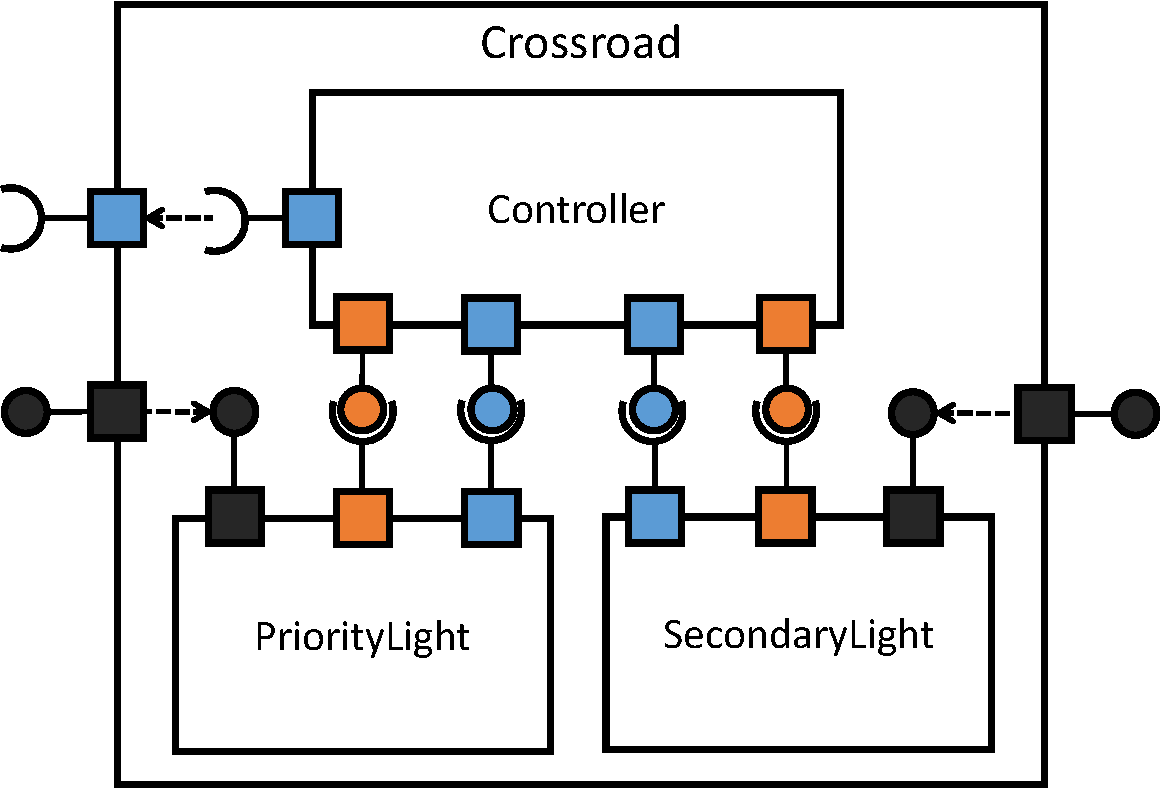
\includegraphics[width=0.52\textwidth]{figures/Controller-gcd.pdf}
	\caption{The synchronous Crossroad composite model composing a Controller and two Traffic light statecharts.}
	\label{fig:crossroads-composite-model}
\end{figure}

\subsubsection{Asynchronous Components}
Asynchronous components represent independently running
component instances. There is no guarantee on the running time or the running frequency of such components. Asynchronous components communicate with each other via ports using buffered \emph{messages}. There are two types of asynchronous components in \gamma: asynchronous composite component and synchronous component wrapper.
\paragraph{Synchronous component wrapper} A synchronous component wrapper wraps a single synchronous component, turning it into an asynchronous component. In addition to the ports of the wrapped component, synchronous component wrappers have ports that are generally used for the reception of control messages. Furthermore, a synchronous component wrapper has one or more
message queues, which store the incoming messages of the component. A message queue has multiple attributes:
\begin{itemize}
	\item \textbf{Capacity} specifies the maximum number of messages that can be stored in the particular
	queue.
	\item \textbf{Priority} specifies the order in which the contents of message queues are retrieved during
	the execution of the asynchronous component. A message is always retrieved from a
	non-empty queue with the highest priority.
	\item \textbf{Event references} specify the types of messages that can be stored in the particular message queue.
\end{itemize}

During execution, messages are retrieved individually from messages queues. A message
is always taken from the highest priority non-empty queue. If the particular message was
received on a port that is implicitly derived from the wrapped component, the message is
converted to a signal (as synchronous components communicate with signals) and transmitted
to the wrapped synchronous component (potentially overwriting previously sent signals). If
it was received on a port explicitly defined on the wrapper component, the message does not
get transmitted.

A synchronous component wrapper also has one or more \emph{control specifications}, which
specify the message types that are able to trigger the execution of the particular component.
If a message with a specified type arrives to the wrapper component, the wrapped synchronous
component may be executed in one of the following ways:
\begin{itemize}
	\item Run once: the wrapped component executes a single cycle.
	\item Run to completion: the wrapped component executes as many cycles as needed to
	ensure all inner signals are processed and no additional steps could be taken.
	\item Reset: the wrapper component gets into its initial state.
\end{itemize}

Furthermore, synchronous component wrappers can contain zero or more clocks, which emit tick
events at defined timed intervals. Currently, seconds and milliseconds are supported as unit of measurements.

The following code snippet presents an example wrapper model, which wraps the previously defined \textsl{CrossroadComponent}. \textsl{AsyncCrossroad} defines a single port \textsl{execution} on which the execution commands
are expected. Messages received on port execution are stored in queue \textsl{execution}, whereas
the messages of additional (implicit) ports are stored in queue \textsl{crossroads}. The priority of
the former is higher. Owing to the control specifications, when a message execute is retrieved,
the wrapped component gets executed for a full step, that is, as many cycles as needed to
process all signals of each contained components of the wrapped component. When either
a clock signal of \textsl{clockSignal} or an interrupt signal of port \textsl{police} is received, the wrapped
component is executed for a single cycle.
\begin{lstlisting}
async AsyncCrossroad of CrossroadComponent [
  // External port of the wrapper
  port execution : requires Executable
] {
  // Clock
  clock clockSignal  ( rate = 100 ms)
  // Control specifications
  when execution.execute / full step
  when clockSignal / run
  when police.interrupt / run
  // Message queues
  queue execution(priority = 2, capacity = 8) {
    execution.execute, clockSignal
  }
  queue crossroads(priority = 1, capacity = 8) {
    police.any, priorityLightOutput.any, secondaryLightOutput.any
  }
}
\end{lstlisting}
\paragraph{Asynchronous composite component}
Asynchronous composite components support the hierarchical definition of asynchronous
components. Similarly to synchronous composite components, an asynchronous composite
component consists of port bindings and channels in addition asynchronous component instances,
which must refer to an asynchronous component as type. It is important to note that
contained composite instances cannot have synchronous components as types in asynchronous
composite components. In such cases, synchronous component wrappers can be used, which
assign asynchronous behavior to synchronous components.

\subsection{Summary}
As a summary of \gamma\ composition modes, Figure \ref{fig:gamma-object-tree} presents the containment hierarchy of an example composite model. Note that the synchronous and asynchronous domain can be bridged only by synchronous composite wrappers. Furthermore, the leaves, which generally define the behavior of composite components, are always statechart definitions.

\begin{figure}[htbp]
	\center
	%	\resizebox{140mm}{!}{
	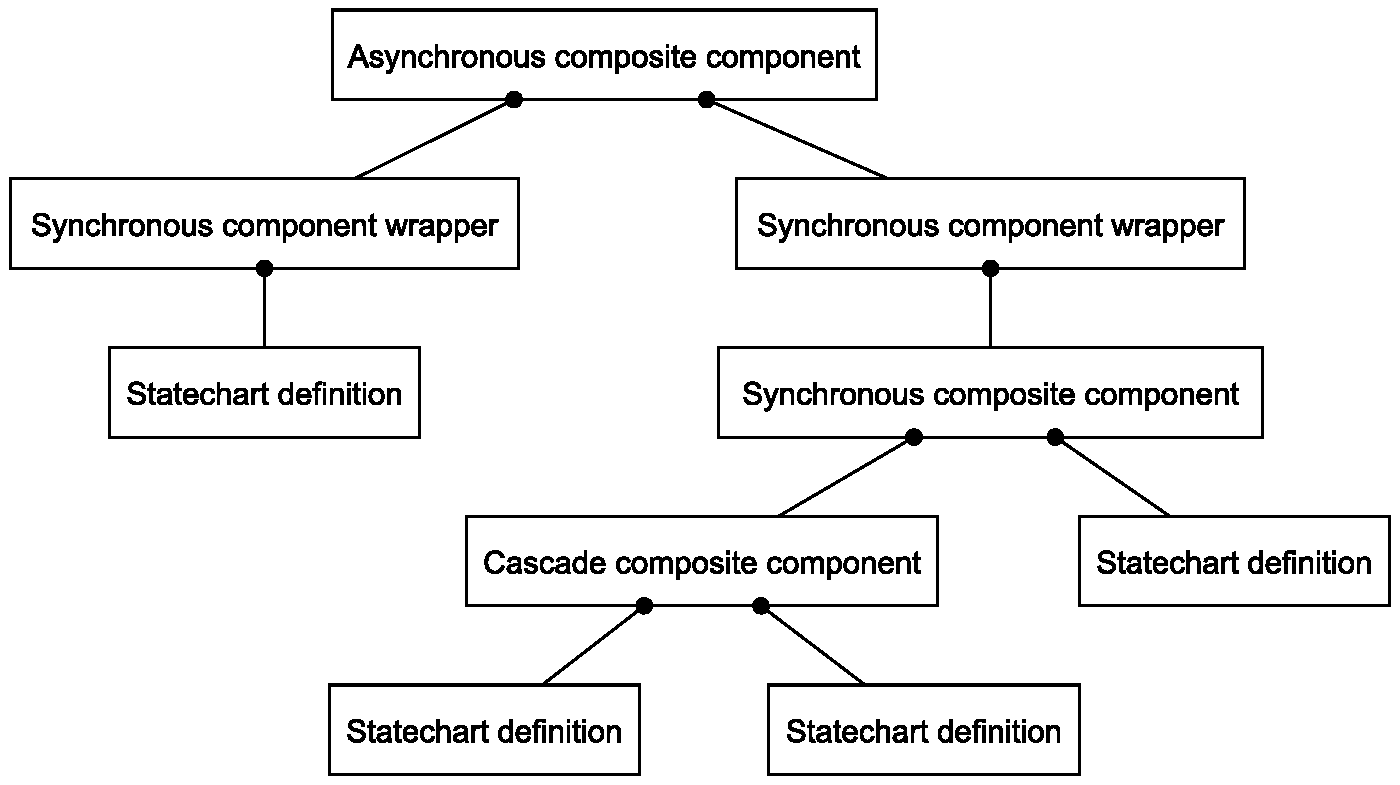
\includegraphics[width=1.0\linewidth]{figures/gamma_object_tree.pdf}
	%	}
	\caption{A composite model hierarchy in \gamma.}
	\label{fig:gamma-object-tree}
\end{figure}

\section{Conclusion and Future Work}
\label{sec:conclusion}
The \framework\ is a modeling tool that supports the development of reactive systems by offering hierarchical composition of statechart components. The three distinguished composition modes are the asynchronous-reactive, the synchronous-reactive and cascade. Asynchronous components represent independently running components, which communicate with immutable messages stored in message queues. This semantics is suitable for designing
separate units executed in their own processes. Synchronous-reactive components are useful for providing a single executing unit consisting of multiple, functionally independent components.
This composition mode is beneficial for the design of low-level controllers. Cascade composition is practical for designing units with pipeline-like behavior: the input given into the model is processed by multiple consecutive filters.

Subject to future work, we plan to extend the code generation and formal verification services of \gamma\ to support the aforementioned composition modes, as currently only the synchronous-reactive composition mode is supported. Code generation can be completed rather easily as we already have detailed plans on how these modeling modes should be implemented. However, the formal analysis of asynchronous-reactive models will be a challenge, as model checkers could not cope with the state space generated by the possible interleaving of dispatched/received messages.

\section*{Acknowledgment}
\begin{figure}[!h]
	\centering
	
\includegraphics[width=0.12\textwidth]{figures/unkp_logo.jpg}
\end{figure}
Supported by the ÚNKP-17-2-I New National Excellence Program of the Ministry of Human Capacities.
